% --------------------------------------------------------------
% This is all preamble stuff that you don't have to worry about.
% Head down to where it says "Start here"
% --------------------------------------------------------------
 
\documentclass[12pt]{article}
 
\usepackage[margin=1in]{geometry} 
\usepackage{amsmath,amsthm,amssymb}
\usepackage[margin=1in]{geometry} 
\usepackage{amsmath,amsthm,amssymb}
\usepackage[english]{babel} 
\usepackage[T1]{fontenc} %escribe lo del teclado
\usepackage[utf8]{inputenc} %Reconoce algunos símbolos
\usepackage{lmodern} %optimiza algunas fuentes
\usepackage{graphicx}
\graphicspath{ {images/} }
\usepackage[urlcolor=blue,colorlinks=true]{hyperref}
\usepackage{makecell}
\usepackage{adjustbox}
\usepackage[justification=centering]{caption}

 
\newcommand{\N}{\mathbb{N}}
\newcommand{\Z}{\mathbb{Z}}
 
\newenvironment{theorem}[2][Theorem]{\begin{trivlist}
\item[\hskip \labelsep {\bfseries #1}\hskip \labelsep {\bfseries #2.}]}{\end{trivlist}}
\newenvironment{lemma}[2][Lemma]{\begin{trivlist}
\item[\hskip \labelsep {\bfseries #1}\hskip \labelsep {\bfseries #2.}]}{\end{trivlist}}
\newenvironment{exercise}[2][Exercise]{\begin{trivlist}
\item[\hskip \labelsep {\bfseries #1}\hskip \labelsep {\bfseries #2.}]}{\end{trivlist}}
\newenvironment{problem}[2][Problem]{\begin{trivlist}
\item[\hskip \labelsep {\bfseries #1}\hskip \labelsep {\bfseries #2.}]}{\end{trivlist}}
\newenvironment{question}[2][Question]{\begin{trivlist}
\item[\hskip \labelsep {\bfseries #1}\hskip \labelsep {\bfseries #2.}]}{\end{trivlist}}
\newenvironment{corollary}[2][Corollary]{\begin{trivlist}
\item[\hskip \labelsep {\bfseries #1}\hskip \labelsep {\bfseries #2.}]}{\end{trivlist}}

\newenvironment{solution}{\begin{proof}[Solution]}{\end{proof}}
 
\begin{document}
 
% --------------------------------------------------------------
%                         Start here
% --------------------------------------------------------------
 
\title{Green Orbital Propulsion System for a Small Satellite}
\author{Christian Molli\`ere}
\maketitle

% B1
\section{Reference Case Definition}
\label{chap:reference_case}
During our internet research the propulsion systems in Table \ref{tab:reference} were found. All systems use monopropellants and are used for AOCS tasks of the spacecraft. In the following we will use the \textbf{XMM Thruster} as a reference case using a chamber pressure of $p_c=5.5\text{bar}-24\text{bar}$ and a nozzle expansion ratio of $\epsilon=60$.\\
 
% B2
\section{Propellants Comparision}
Using the chamber pressure $p_c=5.5\text{bar}-24\text{bar}$ and the nozzle expansion ratio $\epsilon=60$ of the reference case defined in Chapter \ref{chap:reference_case} the following green propellants in Table \ref{tab:comparison} are investigated using NASA CEA. The initial temperature of each propellant is assumed to be $20^\circ\text{C}$.

\begin{table}[h!]
	\centering
	\caption{Comparison of green propellants to the reference case. Each calculation is done using the minimum and maximum feeding pressure of the reference case.}
	\begin{tabular}{|c|c|c|}
		\hline
		Propellant & Vacuum Specific Impulse {[}s{]} & Combustion Temperature {[}K{]} \\ \hline
		LMP-103S   & 253.3                         & 1865                      \\ \hline
		AF-M315E   & 261                         & 2102-2105                      \\ \hline
		H2O2, 98\% & 188                         & 1225                      \\ \hline     
	\end{tabular}
	\label{tab:comparison}
\end{table}

% B3
\section{Propellant Optimization}
To optimize the propellant composition of Methanol, ADN and Water a rocketCEA script was written in Python. It performs a search on a composition grid, with a step size of $1\%$ weight fraction. It iterates through all possible composition permutations. We assume the chamber pressure to be again $24\text{bar}$, the expansion ratio to be $\epsilon=60$ and the initial propellant temperature of the composition to be $T_0=20^{\circ}C$. The results are discussed in the following.

\paragraph{First results}
The top figure in Figure \ref{fig:fuel_optimization_all_results} shows the result of this optimization with a maximum $I_{sp}=302.29s$ using $83\%$ of Methanol, $17\%$ ADN and no Water.

\begin{figure}[!h]
	\centering
	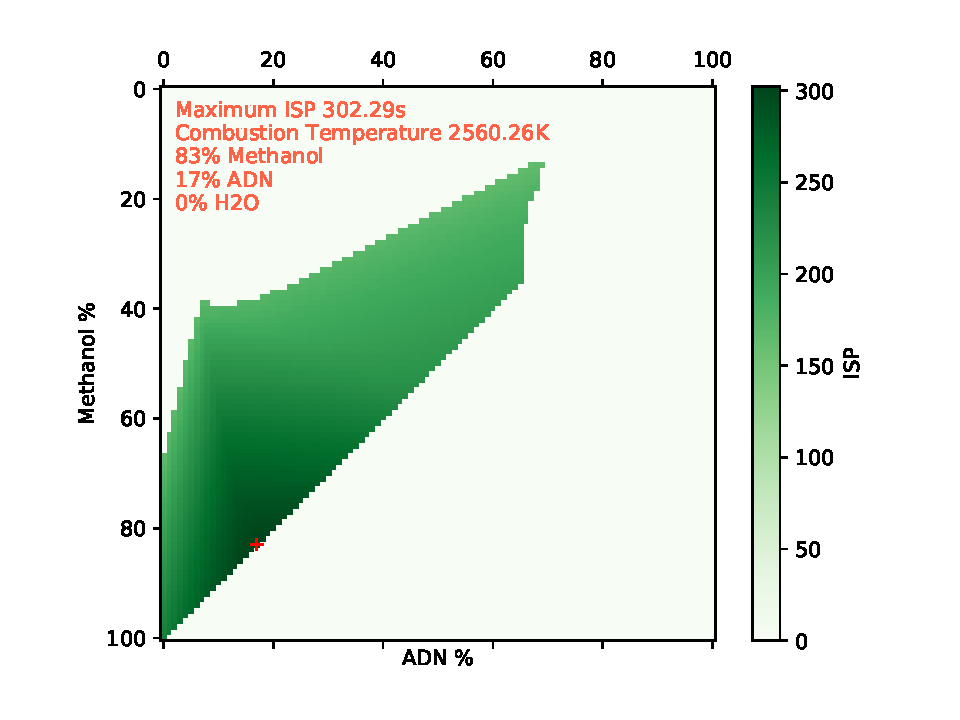
\includegraphics[width=0.8\linewidth]{figures/b2_1.pdf}
	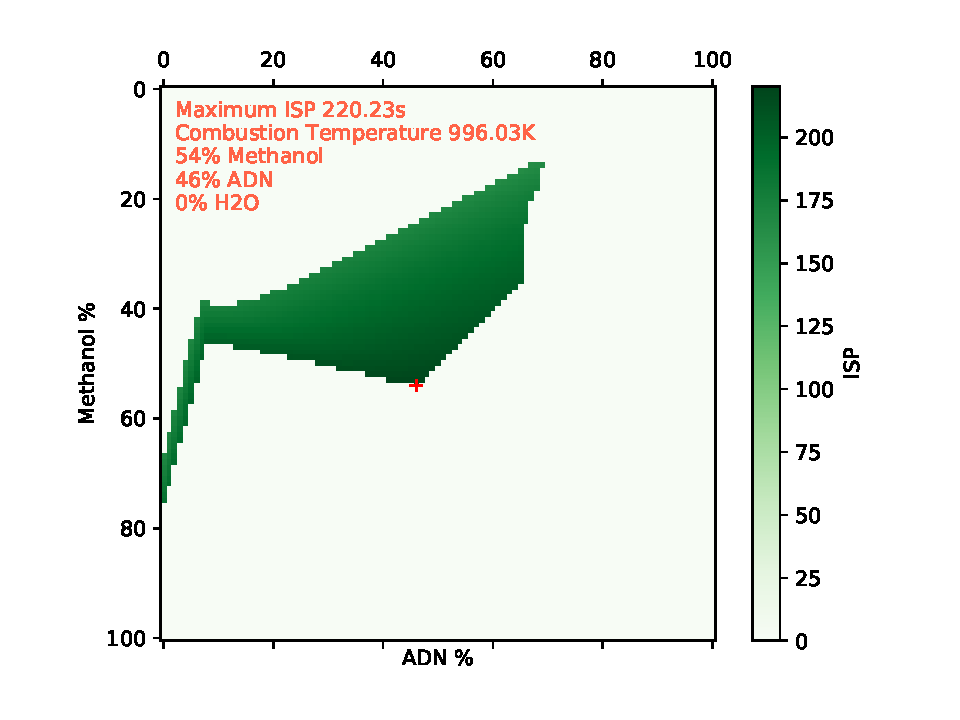
\includegraphics[width=0.8\linewidth]{figures/b2_2.pdf}
	\caption{Figure showing the fuel optimization using Nasa CEA to compute the highest possible ISP (top). The best results are highlighted with a red cross. The second figure shows the best result after all reactions with a combustion temperature above 1000$^\circ$C are cut (bottom).}
	\label{fig:fuel_optimization_all_results}
\end{figure}

\paragraph{Considering combustion temperature and solubility}
Since the task is to find a propellant composition with a combustion temperature below 1000$^\circ$C we cut all results that do not comply with this boundary condition. The result is shown in the lower Figure \ref{fig:fuel_optimization_all_results} with a maximum $I_{sp}=220.23s$ using $54\%$ of Methanol, $46\%$ ADN and no Water.\\

Furthermore, we need to consider that the solid ADN will need to be dissolved in the other two components of the propellant. At a temperature of $20^\circ C$, which is coherent with our initial propellant temperature, $3.56$ times more Water than ADN is needed to completely dissolve the ADN. Methanol can dissolve much more ADN at a rate of only $0.86$ \cite{Larsson2011}. 
\begin{equation}
	\frac{wt\%_{\text{Methanol}}}{wt\%_{\text{ADN}}} = \frac{54\%}{46\%} = 1.174 \geq 0.86
	\label{eq:solubility}
\end{equation}
According to equation \ref{eq:solubility} the amount of Methanol in our result is sufficient to completely dissolve the used ADN. Adding water will only lower the $I_{sp}$ of the propellant composition. Therefore, the final result is chosen to be at $54\%$ of Methanol, $46\%$ ADN and no Water.

% TODO QUELLEN IN BIB FILE


% B4
\section{Thruster Preliminary Design}

% B5
\section{Detailed Design Blow-Down Feed System}

% Overview
\newpage
\begin{adjustbox}{angle=90, center,caption={Overview of small propulsion systems using monopropellants.},float=table}
	\begin{tabular}{|c|c|c|c|c|c|c|}
		\hline
		Name & Propellants & \makecell{Number of\\Thrusters} & \makecell{Thruster\\Class {[}N{]}} & \makecell{Total\\Impulse [Ns]} & Other & Reference\\ \hline
		\makecell{XMM\\Thruster} & N2H4 & 8 & 20 & \makecell{$>517000$}  & \makecell{$I_{sp}=222-230s$,\\$p_c=5.5-24\text{bar}$,\\$\epsilon=60$} & \makecell{ \href{http://www.esa.int/esapub/br/br250/br250.pdf}{ESA Doc, Page 209;}\\\href{http://www.space-propulsion.com/spacecraft-propulsion/hydrazine-thrusters/20n-hydrazine-thruster.html}{Ariane Group}} \\ \hline
		\makecell{TanDEM-X\\Thruster} & \makecell{N2H4} & 4 & 1 & \makecell{$>135000$}& \makecell{$I_{sp}=200-223s$,\\$p_c=5.5-22\text{bar}$,\\$\epsilon=80$\\} & \makecell{\href{https://www.researchgate.net/profile/Ralph_Kahle/publication/259897316_Flight_Dynamics_Operations_of_the_TanDEM-X_Formation/links/0a85e53c3b917d441a000000/Flight-Dynamics-Operations-of-the-TanDEM-X-Formation.pdf}{FD TanDEM-X};\\\href{http://www.space-propulsion.com/spacecraft-propulsion/hydrazine-thrusters/1n-hydrazine-thruster.html}{Ariane Group}}\\ \hline
		\makecell{Prisma\\Thruster}& LMP-103S & 2 & 1 & \makecell{$\approx 108773$\footnote{Calculatted from $I_{\text{sp}}\cdot g_0\cdot m_p\cdot n_{\text{Thruster}}$}} & \makecell{$I_{sp}=204-231s$,\\$p_c=4.5-22\text{bar}$,\\$\epsilon=100$} & \href{http://ecaps.space/products-1n.php}{1N HPGP Thruster}                                                                                                                                                                                       \\ \hline
	\end{tabular}
	\label{tab:reference}
\end{adjustbox}

% References
\newpage
\bibliography{references/papers.bib} 
\bibliographystyle{ieeetr}
 
\end{document}